For a simple Lie algebra of dimension $d$, we defined the set of $r$ roots $\alpha$ in some set $\Phi$ of size $|\Phi|=d-r$. In particular, we showed that the roots $\alpha$ not only lie in the dual space to the Cartan subalgebra $\fh^*$ but indeed they form a basis for $\fh^*$.

That is, a basis for $\fh^*$ is given by
$$B=\set{\alpha_{(i)},i=1,\ldots,r,\alpha_{(i)}\in \Phi}.$$
Now for a generic element $\beta \in \Phi$, it can be decomposed into its components
$$\beta=\sum_{i=1}^r \beta^i \alpha_{(i)}$$ where the coefficients are in general complex, $\beta^i\in \CC$. We further reasoned that
$$(\beta,\alpha_{(j)})=\sum_{i=1}^r \beta^i \underbrace{(\alpha_{(i)},\alpha_{(j)})}_{(\kappa^{-1})_{ij}}.$$
But since the entries of $\kappa^{-1}$ are real and $(\alpha,\beta)\in \RR \forall \alpha,\beta \in \RR,$ this tells us that
$$\forall \beta \in \Phi, \beta \in \fh^*_\RR =\text{Span}_\RR \set{\alpha_{(i)},i=1,\ldots,r}.$$
That is, a generic element of $\fh^*$ lies in the real span of the roots.

Not consider the inner product of two general elements of the dual space, $\lambda,\mu \in \fh^*_\RR.$
\begin{align*}
    \lambda&= \sum_{i=1}^r \lambda^i \alpha_{(i)} \in \fh^*_\RR\\
    \mu&= \sum_{i=1}^r \mu^i \alpha_{(i)} \in \fh^*_\RR,
\end{align*}
with $\lambda^i,\mu^i \in \RR$ (since these elements are in $\fh^*_\RR$ and therefore in the real span).

But this means that their inner product also lies in the real span of the roots,
$$(\lambda,\mu)=\sum_{i,j=1}^r \lambda^i \mu^i (\alpha_{(i)}, \alpha_{(j)})\in \RR.$$
However, we also recall that the inner product of a vector with itself can be written as
$$(\lambda,\lambda)=\frac{1}{N}\sum_{\delta\in \Phi}\lambda^i \delta^i \delta^j \lambda_j =\frac{1}{N}\sum_{\delta \in \Phi}(\lambda,\delta)^2.$$
But now we see that since this inner product is a sum of squares of real numbers, $(\lambda,\lambda)\geq 0$ with equality iff $(\lambda,\delta)=0\forall \delta \in \Phi$. But by the non-degeneracy of the inner product, we see that there can be no element that is orthogonal to all other elements of $\Phi$ unless that element is the zero element, i.e.
$$(\lambda,\lambda)=0\iff \lambda=0.$$

To summarize, we've recovered many of the nice properties of Euclidean space on the roots. The roots $\alpha\in \Phi$ live in a real vector space $\fh^*_\RR \simeq \RR^r$, such that $\forall \lambda,\mu\in \fh^*_\RR$, the following properties hold:
\begin{enumerate}
    \item $(\lambda,\mu)\in \RR$
    \item $(\lambda,\lambda)\geq 0$
    \item $(\lambda,\lambda)=0\iff \lambda=0$,
\end{enumerate}
which means that $\fh^*_\RR$ admits a Euclidean inner product $(\cdot,\cdot)$.

Since $(\alpha,\alpha)>0 \forall \alpha \in \Phi$, we can therefore define a \emph{length} of a root defined as
$$|\alpha|\equiv +(\alpha,\alpha)^{1/2} >0,$$
and thus an ``angle'' $\phi$ between two roots, which takes the standard form
$$(\alpha,\beta)=|\alpha||\beta|\cos \phi$$
with $\phi\in[0,\pi]\forall \alpha,\beta\in \Phi.$

However, we also recall that there was an integer quantization condition on the inner products, which we may write as
\begin{align}
    \frac{2(\alpha,\beta)}{(\alpha,\alpha)}&=\frac{2|\beta|}{|\alpha|}\cos\phi \in \ZZ\\
    \frac{2(\beta,\alpha)}{(\alpha,\alpha)}&=\frac{2|\alpha|}{|\beta|}\cos\phi \in \ZZ.
\end{align}
We can of course multiply these two RHS expressions together to get another integer, and we find that
$$4\cos^2\phi \in \ZZ,$$ which tells us that
$$\cos\phi = \pm \frac{\sqrt{n}}{2}$$ where $n\in\set{0,1,2,3,4}$.

Thus we have $\phi=0,\pi/2,\pi$ corresponding to $\alpha=\beta,(\alpha,\beta)=0,\alpha=-\beta$. We also have other possible values for $\phi$: when $\phi=\pi/6,\pi/4, \pi/3,$ then $(\alpha,\beta)>0$, while when $\phi=2\pi/3,3\pi/4,5\pi/6,$ then $(\alpha,\beta)<0$. To recap, not only can we define angles between two roots $\alpha,\beta$, but these angles are also constrained to a finite set.

\begin{figure}
    \centering
    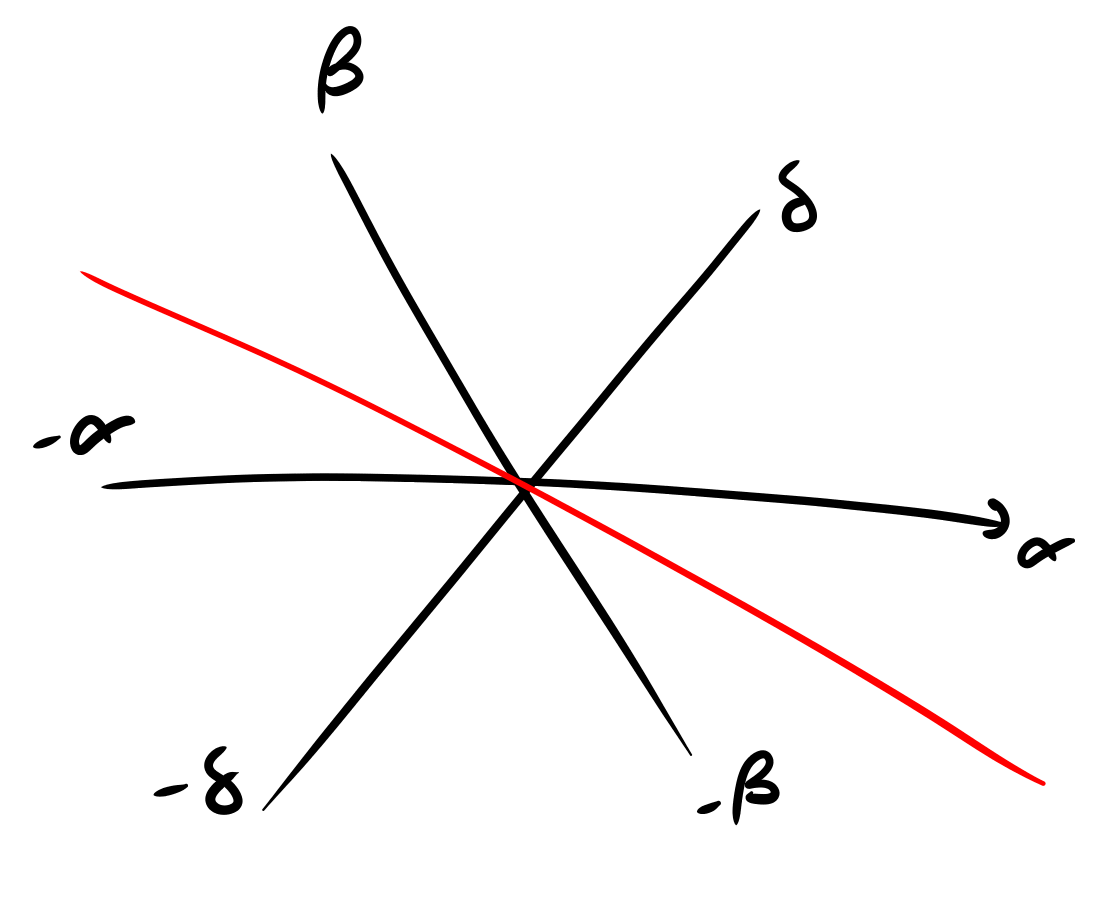
\includegraphics{2018/11/20181113_simpleroots.png}
    \caption{An illustration of the division of simple roots into two sets, $\Phi_+$ and $\Phi_-$. The red line represents the hyperplane, and $\alpha,\beta,\delta$ are roots in $\Phi$. $\Phi_+$ lies above the red line and $\Phi_-$ below.}
    \label{fig:simpleroots}
\end{figure}

\subsection*{Simple roots} Let us divide the roots $\alpha\in \Phi$ into positive and negative by a hyperplane in $\fh^*.$ This hyperplane divides our set of roots $\Phi$ into
$$\Phi=\Phi_+ \cup \Phi_-$$
but is otherwise arbitrary. See Fig. \ref{fig:simpleroots} for an illustration. We can always construct such a plane by picking any plane that is not coplanar with any root (if it is, just move the plane a bit) and labeling all the roots on one side to be the $+$ roots and all the roots on the other to be $-$. Therefore
$\forall \alpha,\beta \in \Phi$, we get the following nice properties:
\begin{enumerate}
    \item $\alpha\in \Phi_+\iff -\alpha \in \Phi_-$
    \item $\alpha,\beta \in \Phi_+$ and $\alpha + \beta \in \Phi \implies \alpha+\beta \in \Phi_+$ (and similarly $\alpha,\beta\in \Phi_-, \alpha+\beta\in \Phi \implies \alpha+\beta \in \Phi_-$).
\end{enumerate}

\begin{defn}
We now say that a \term{simple root} is a positive root which cannot be written as the sum of two positive roots, i.e.
$$\delta \in \Phi_S \text{ (is simple)} \iff \delta \in \Phi_+, \delta \neq \alpha+\beta \text{ for any } \alpha,\beta \in \Phi_+.$$
\end{defn}
Simple roots have some good properties.
\begin{enumerate}
    \item[i)] if $\alpha,\beta\in \Phi_S$, then $\alpha=\beta$ is not a root. For suppose $\alpha-\beta\in \Phi$. Then either
    \begin{itemize}
        \item $\alpha-\beta \in \Phi_+$. Then $\alpha=\alpha-\beta+\beta \implies \alpha$ not simple.
        \item $\alpha-\beta \in\Phi_-$. Then $\beta=\beta-\alpha+\alpha \implies \beta$ not simple.
    \end{itemize}
    Either way, we reach a contradiction, so $\alpha-\beta\notin \Phi.$
    \item[ii)] If $\alpha,\beta \in \Phi_S,$ then the $\alpha$-string through $\beta$ ($\a\neq \beta$) takes the form
    $$l_{\a,\beta}=1-\frac{2(\a,\beta)}{(\a,\a)}\in \NN.$$
    \begin{proof} The string consists of roots
    $$S_{\a,\beta}=\set{\beta+n\alpha;n\in \ZZ\quad n_- \leq n \leq n_+}.$$
    But this set certainly contains at least one element-- $\beta$, with $n=0$. Therefore $n_+\geq 0$ and $n_-\leq 0$. However, we also know that the sum of the bounds $n_+,n_-$ is given by 
    $$(n_++n_-)=-\frac{2(\a,\beta)}{(\a,\a)}\in \ZZ.$$
    Since $\a,\beta$ are simple roots, $\beta-\alpha \notin \Phi \implies n_- =0$. Thus
    $$n_+ = -\frac{2(\alpha,\beta)}{(\a,\a)}\in \ZZ_{\geq 0}.$$
    We conclude that the root string takes the form
    $$l=n_+ - n_- + 1 = n_+ +1 = 1-\frac{2(\a,\beta)}{(\a,\a)} \in \NN.$$
    \end{proof}
    \item[iii)] $\forall \alpha,\beta \in \Phi_S, \alpha \neq \beta$, we have $(\alpha,\beta)\leq 0$. (This follows from the previous property about the root string and the positivity of $(\alpha,\alpha)$.)
    \item[iv)] Any positive root $\beta\in \Phi_+$ can be written as a linear combination of simple roots with positive integer coefficients.
    \begin{proof}
    This is trivially true if $\beta\in \Phi_S$ is itself a simple root. If $\beta\notin \Phi_S$, then we can write $\beta=\beta_1+\beta_2$ where $\beta_1,\beta_2 \in \Phi_+.$ If $\beta_1,\beta_2\in \Phi_S$, then we are done. Otherwise, we can split $\beta_1=\beta_3,\beta_4$ where $\beta_3,\beta_4\in \Phi_+$. The set of roots is of finite dimension, so this process has to terminate eventually with a full decomposition of $\beta$ into simple roots.
    \end{proof}
    \item[v)] Simple roots are linearly independent.
    \begin{proof}
    Consider vectors $\lambda\in \fh^*_\RR$ which can be written in terms of the $\alpha_{(i)}$ basis elements. Thus
    $$\lambda=\sum_{i\in J} c_i \alpha_{(i)}$$
    with $J$ a set of indices, $\alpha_{(i)}\in \Phi_S$, and $c_i\in \RR$. We can split $J$ into $J=J_+ \cup J_-$ where
    $$J_+=\set{i\in J: c_i >0},J_-=\set{i\in J: c_i <0}$$
    We'll finish the proof next time.
    \end{proof}
\end{enumerate}
%add the cross-references here! Check the notes